\documentclass[12pt]{article}
\usepackage[table]{xcolor}
\usepackage[shortlabels]{enumitem}
\usepackage{tabularx,xltabular}
\usepackage{graphicx}
\usepackage{hyperref}
\usepackage{verbatim}
\usepackage{geometry}
\usepackage{ulem}
\usepackage[official]{eurosym}
\usepackage{tikz}
\usetikzlibrary{arrows,backgrounds,calc,decorations.markings,patterns,3d}
\usepackage{pgfplots}
\pgfplotsset{compat = newest}
\usetikzlibrary{fit}
\newcommand\addvmargin[1]{
\usetikzlibrary{arrows}
\node[fit=(current bounding box),inner ysep=#1,inner xsep=0]{};}
\usepackage{cancel}
\usepackage{fontspec}
\usepackage{array}  
\geometry{a4paper, top=2cm, left=2cm, right=2cm, bottom=2cm, headsep=1cm}
\usepackage{tabu}
\usepackage{pst-node}
\usepackage{colortbl}
\usepackage{array}
\usepackage{german}
\setlength\parindent{0pt}
\newcolumntype{?}{!{\vrule width 1pt}}
\usepackage{makecell}
\renewcommand{\arraystretch}{2.5}
\usepackage{pbox}
\usepackage{amssymb}
\usepackage{amsmath}
\usepackage{booktabs}
\newcolumntype{L}[1]{>{\raggedright\let\newline\\\arraybackslash\hspace{0pt}}m{#1}}
\newcolumntype{C}[1]{>{\centering\let\newline\\\arraybackslash\hspace{0pt}}m{#1}}
\newcolumntype{R}[1]{>{\raggedleft\let\newline\\\arraybackslash\hspace{0pt}}m{#1}}
\begin{document}
\rightline{Datum: 12.06.2023}
\centerline{{\Large Tägliche Übungen}} 
\vspace{1cm}
\noindent \\


\begin{xltabular}{\textwidth}{|C{0.75cm}|X|C{0.75cm}|X|}
\arrayrulecolor{black}\hline
a)&Berechne die Variable $$-7-1\cdot a-2+3\cdot a=-1$$
&
b)&Berechne die Variable $$12-25-1\cdot b+8\cdot b=29$$
\\\hline
c)&Berechne die Variable $$1\cdot y-3+1\cdot y-13=-4$$
&
d)&Berechne die Variable $$-7+3\cdot a+6\cdot a-12=-1$$
\\\hline
e)&Berechne die Variable $$5\cdot b-10+5\cdot b+3=103$$
&
f)&Berechne die Variable $$-2\cdot x-15+1+9\cdot x=42$$
\\\hline
\end{xltabular}
\vspace{0.5cm}
\newpage
\rightline{Datum: 12.06.2023}
\centerline{{\large Lösungen Tägliche Übungen}} 
\vspace{0.5cm}

\begin{xltabular}{\textwidth}{|C{0.75cm}|X|C{0.75cm}|X|}
\arrayrulecolor{black}\hline
a)&\begingroup\setlength{\jot}{-0.03cm}
\tikzstyle{background grid}=[draw, black!15,step=.5cm]
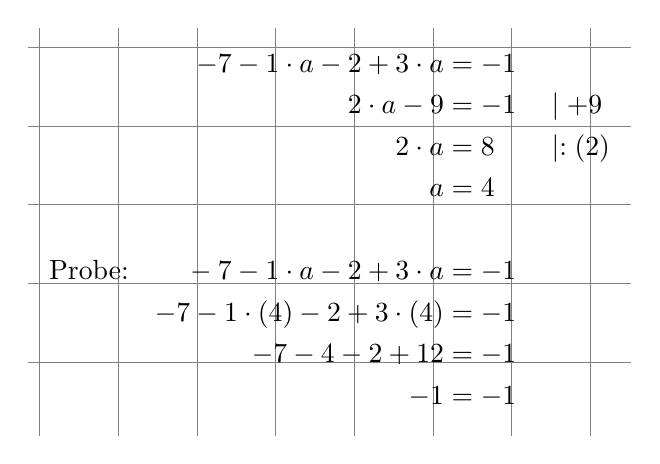
\begin{tikzpicture}[show background grid]
\node[below right] at (0,0.1) {
$\begin{aligned}
-7-1\cdot a-2+3\cdot a &=-1& &  \\
2\cdot a - 9 &=-1& & \mid + 9\\
2\cdot a &=8& & \mid :\left(2\right)\\
a &=4& & 
\\
\\
\mbox{Probe:}\qquad -7-1\cdot a-2+3\cdot a &=-1& &  \\
-7-1\cdot \left(4\right)-2+3\cdot \left(4\right) &=-1& &  \\
-7-4-2+12 &=-1& &  \\
-1 &=-1& &  \\
\end{aligned}$};
\end{tikzpicture}
\endgroup
&
b)&\begingroup\setlength{\jot}{-0.03cm}
\tikzstyle{background grid}=[draw, black!15,step=.5cm]
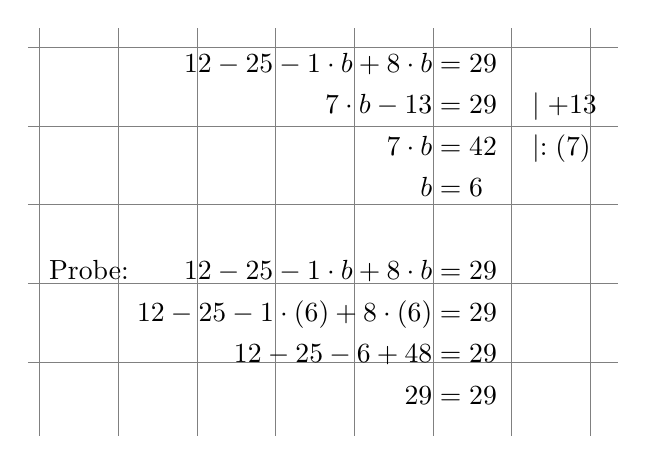
\begin{tikzpicture}[show background grid]
\node[below right] at (0,0.1) {
$\begin{aligned}
12-25-1\cdot b+8\cdot b &=29& &  \\
7\cdot b - 13 &=29& & \mid + 13\\
7\cdot b &=42& & \mid :\left(7\right)\\
b &=6& & 
\\
\\
\mbox{Probe:}\qquad 12-25-1\cdot b+8\cdot b &=29& &  \\
12-25-1\cdot \left(6\right)+8\cdot \left(6\right) &=29& &  \\
12-25-6+48 &=29& &  \\
29 &=29& &  \\
\end{aligned}$};
\end{tikzpicture}
\endgroup
\\\hline
c)&\begingroup\setlength{\jot}{-0.03cm}
\tikzstyle{background grid}=[draw, black!15,step=.5cm]
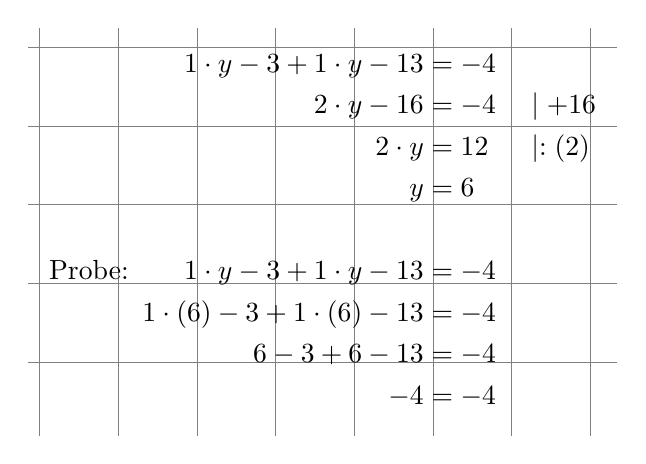
\begin{tikzpicture}[show background grid]
\node[below right] at (0,0.1) {
$\begin{aligned}
1\cdot y-3+1\cdot y-13 &=-4& &  \\
2\cdot y - 16 &=-4& & \mid + 16\\
2\cdot y &=12& & \mid :\left(2\right)\\
y &=6& & 
\\
\\
\mbox{Probe:}\qquad 1\cdot y-3+1\cdot y-13 &=-4& &  \\
1\cdot \left(6\right)-3+1\cdot \left(6\right)-13 &=-4& &  \\
6-3+6-13 &=-4& &  \\
-4 &=-4& &  \\
\end{aligned}$};
\end{tikzpicture}
\endgroup
&
d)&\begingroup\setlength{\jot}{-0.03cm}
\tikzstyle{background grid}=[draw, black!15,step=.5cm]
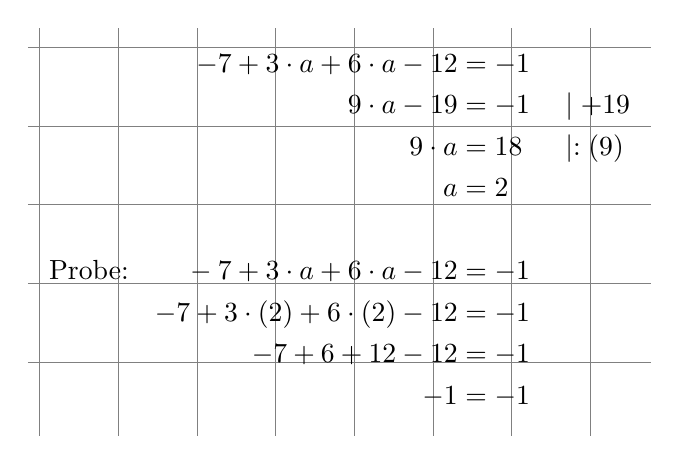
\begin{tikzpicture}[show background grid]
\node[below right] at (0,0.1) {
$\begin{aligned}
-7+3\cdot a+6\cdot a-12 &=-1& &  \\
9\cdot a - 19 &=-1& & \mid + 19\\
9\cdot a &=18& & \mid :\left(9\right)\\
a &=2& & 
\\
\\
\mbox{Probe:}\qquad -7+3\cdot a+6\cdot a-12 &=-1& &  \\
-7+3\cdot \left(2\right)+6\cdot \left(2\right)-12 &=-1& &  \\
-7+6+12-12 &=-1& &  \\
-1 &=-1& &  \\
\end{aligned}$};
\end{tikzpicture}
\endgroup
\\\hline
e)&\begingroup\setlength{\jot}{-0.03cm}
\tikzstyle{background grid}=[draw, black!15,step=.5cm]
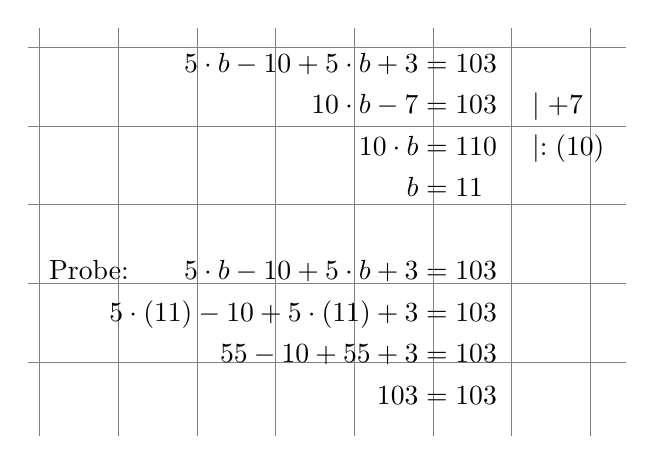
\begin{tikzpicture}[show background grid]
\node[below right] at (0,0.1) {
$\begin{aligned}
5\cdot b-10+5\cdot b+3 &=103& &  \\
10\cdot b - 7 &=103& & \mid + 7\\
10\cdot b &=110& & \mid :\left(10\right)\\
b &=11& & 
\\
\\
\mbox{Probe:}\qquad 5\cdot b-10+5\cdot b+3 &=103& &  \\
5\cdot \left(11\right)-10+5\cdot \left(11\right)+3 &=103& &  \\
55-10+55+3 &=103& &  \\
103 &=103& &  \\
\end{aligned}$};
\end{tikzpicture}
\endgroup
&
f)&\begingroup\setlength{\jot}{-0.03cm}
\tikzstyle{background grid}=[draw, black!15,step=.5cm]
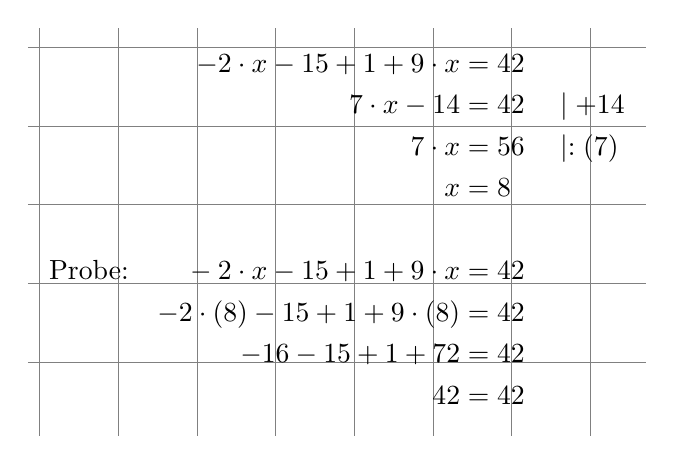
\begin{tikzpicture}[show background grid]
\node[below right] at (0,0.1) {
$\begin{aligned}
-2\cdot x-15+1+9\cdot x &=42& &  \\
7\cdot x - 14 &=42& & \mid + 14\\
7\cdot x &=56& & \mid :\left(7\right)\\
x &=8& & 
\\
\\
\mbox{Probe:}\qquad -2\cdot x-15+1+9\cdot x &=42& &  \\
-2\cdot \left(8\right)-15+1+9\cdot \left(8\right) &=42& &  \\
-16-15+1+72 &=42& &  \\
42 &=42& &  \\
\end{aligned}$};
\end{tikzpicture}
\endgroup
\\\hline
\end{xltabular}
\vspace{0.5cm}
\end{document}